\documentclass[a4paper,11pt]{article}
\usepackage[T1]{fontenc}\usepackage[utf8]{inputenc}\usepackage{lmodern}\usepackage{microtype}
\usepackage[a4paper,margin=1in,headheight=15pt,headsep=14pt]{geometry}
\usepackage{amsmath,amssymb}\usepackage{graphicx}\usepackage{booktabs}
\usepackage[table,svgnames]{xcolor}\usepackage[most]{tcolorbox}\tcbuselibrary{skins,breakable}
\usepackage{tikz}\usepackage{pifont}\usepackage{bbding}\usepackage{enumitem}
\setlist{leftmargin=1.5em,topsep=4pt,itemsep=3pt}\usepackage{parskip}
\usepackage{fancyhdr}\usepackage{titlesec}\usepackage[hidelinks]{hyperref}\usepackage{xurl}
\hypersetup{breaklinks=true}
\definecolor{navy}{HTML}{21355E}\definecolor{navyrule}{HTML}{21355E}
\definecolor{inktext}{HTML}{1A202C}\definecolor{mutedtext}{HTML}{6B7280}
\definecolor{intuFrame}{HTML}{2C5AA0}\definecolor{intuFill}{HTML}{F4F7FC}
\definecolor{everyFrame}{HTML}{8A5A1E}\definecolor{everyFill}{HTML}{FBF1E3}
\definecolor{workFrame}{HTML}{2E7D52}\definecolor{workFill}{HTML}{F1F8F3}
\definecolor{watchFrame}{HTML}{B23A48}\definecolor{watchFill}{HTML}{FBF1F2}
\definecolor{keyFrame}{HTML}{6A4C93}\definecolor{keyFill}{HTML}{F4F0F9}
\color{inktext}\hypersetup{linkcolor=navy,urlcolor=navy,citecolor=navy}
\tcbset{housecallout/.style 2 args={enhanced,breakable,colback=#2,colframe=#1,boxrule=0.6pt,arc=2.4pt,outer arc=2.4pt,left=10pt,right=10pt,top=9pt,bottom=9pt,before skip=11pt,after skip=11pt,fontupper=\normalsize,coltitle=white,fonttitle=\bfseries\sffamily\small,attach boxed title to top left={xshift=6mm,yshift=-3mm},boxed title style={colback=#1,colframe=#1,rounded corners,arc=3pt,boxrule=0pt,left=6pt,right=6pt,top=2pt,bottom=2pt}}}
\newtcolorbox{intuition}{housecallout={intuFrame}{intuFill},title={\raisebox{-0.05ex}{\Pointinghand}\,\ The intuition}}
\newtcolorbox{everyday}{housecallout={everyFrame}{everyFill},title={\raisebox{-0.05ex}{$\bigstar$}\,\ Everyday picture}}
\newtcolorbox{worked}[1]{housecallout={workFrame}{workFill},title={\raisebox{-0.05ex}{\Pencil}\,\ Worked example: #1}}
\newtcolorbox{watchout}{housecallout={watchFrame}{watchFill},title={\raisebox{-0.05ex}{\ding{55}}\,\ Watch out}}
\newtcolorbox{keytake}{housecallout={keyFrame}{keyFill},title={\raisebox{-0.05ex}{\ding{51}}\,\ Key takeaway}}
\newcommand{\CourseShort}{SEML Companion}\newcommand{\SessionNo}{3}\newcommand{\LectureTitle}{Requirements Engineering for ML}
\pagestyle{fancy}\fancyhf{}
\fancyhead[L]{\footnotesize\color{mutedtext}\textsf{\CourseShort}}
\fancyhead[R]{\footnotesize\color{mutedtext}\textsf{Session \SessionNo\ \textperiodcentered\ \LectureTitle}}
\fancyfoot[C]{\footnotesize\color{mutedtext}\thepage}
\renewcommand{\headrulewidth}{0.4pt}\renewcommand{\footrulewidth}{0pt}
\renewcommand{\headrule}{\hbox to\headwidth{\color{navyrule!55}\leaders\hrule height \headrulewidth\hfill}}
\titleformat{\section}{\sffamily\Large\bfseries\color{navy}}{\thesection}{0.8em}{}[{\vspace{2pt}\color{navy!70}\titlerule[0.8pt]}]
\titleformat{\subsection}{\sffamily\large\bfseries\color{navy!92}}{\thesubsection}{0.7em}{}
\titlespacing*{\section}{0pt}{16pt}{8pt}\titlespacing*{\subsection}{0pt}{12pt}{4pt}
\newcommand{\titlebanner}[4]{\begin{tcolorbox}[enhanced,breakable=false,colback=navy,colframe=navy,boxrule=0pt,arc=3pt,outer arc=3pt,left=16pt,right=16pt,top=16pt,bottom=16pt,before skip=2pt,after skip=14pt,width=\linewidth]{\sffamily\footnotesize\bfseries\color{white!85}\MakeUppercase{#1}}\par\vspace{6pt}{\sffamily\bfseries\fontsize{30}{34}\selectfont\color{white}#2\par}\vspace{5pt}{\sffamily\large\color{white!88}#3\par}\vspace{9pt}{\color{white!55}\rule{\linewidth}{0.4pt}}\par\vspace{6pt}{\sffamily\footnotesize\color{white!82}#4\par}\end{tcolorbox}}
\newcommand{\vocab}[1]{\textbf{\color{navy}#1}}
\begin{document}
\thispagestyle{fancy}
\titlebanner{AIMLCZG546 · Session 3 · Companion Reader}{Requirements Engineering for ML Systems}{When to Use ML, Goals, GR4ML Notation, and Measuring Success}{Session 3 · Read alongside the lecture slides · Every concept explained step by step}

\noindent\textbf{How to use this companion.} \textcolor{intuFrame}{\textbf{Blue}} = core intuition. \textcolor{everyFrame}{\textbf{Amber}} = everyday analogy. \textcolor{workFrame}{\textbf{Green}} = worked scenario. \textcolor{watchFrame}{\textbf{Red}} = pitfall. \textcolor{keyFrame}{\textbf{Purple}} = the one line to remember. The running example throughout is a \emph{credit risk prediction system} at a bank.

%==============================================================
\section{When to Use ML}
%==============================================================

ML is a powerful tool, but it is not the right tool for every problem. Geoff Hulten's framework identifies three situations where ML genuinely outperforms rule-based approaches.

\begin{intuition}
A screwdriver is perfect for screws but terrible for nails. ML is perfect for certain types of problems. Using it on the wrong problem wastes months of effort and produces worse results than simpler alternatives.
\end{intuition}

\subsection{Case 1: Intrinsically Hard Problems}

Human language understanding is a canonical example. Consider sarcasm: ``Oh great, another Monday.'' A rule-based system sees the word ``great'' and classifies this as positive sentiment. A human immediately understands it is negative. Language is contextual, ambiguous, culturally loaded, and constantly evolving. No finite set of hand-crafted rules can capture this. ML models learn the patterns from millions of examples.

\subsection{Case 2: Big Problems (Scale)}

Recommending the right song from 100 million tracks to 500 million users, based on each user's listening history, mood, and time of day, is mathematically intractable for a human writing rules. ML can learn a personalised embedding space for every user and every song and compute recommendations in milliseconds.

\subsection{Case 3: Time-Changing Problems}

Fraud patterns evolve. As soon as a rule-based fraud system blocks a particular attack vector, fraudsters adapt. An ML model that retrains weekly on the latest fraud cases continuously adapts to new attack patterns --- a fixed rule set does not.

\begin{everyday}
Case 1 is like asking a human to sort mail by handwriting style across a million letters --- too subjective for rules. Case 2 is like building a menu for every customer in a billion-person restaurant --- too large for manual rules. Case 3 is like a lock that automatically changes its combination when someone figures it out.
\end{everyday}

\begin{watchout}
Using ML on a simple, deterministic problem is a mistake. If a business rule can be written clearly (``if age < 18, block purchase''), write the rule. ML adds cost, complexity, and uncertainty you do not need.
\end{watchout}

\noindent\textbf{Where this shows up in ML/AI.} Every ML project starts with a justification: \emph{why ML and not a rule?} The answer must fall into one of Hulten's three cases, or the project should be reconsidered.

%==============================================================
\section{Requirements Engineering for ML Systems}
%==============================================================

\vocab{Requirements Engineering (RE)} is the process of discovering, documenting, and managing what a system must do and how well it must do it. Traditional RE is straightforward: systems are deterministic. An ML system is probabilistic, data-dependent, and continuously changing, which makes RE significantly harder.

\begin{center}
\resizebox{\linewidth}{!}{%
\begin{tabular}{lll}
\toprule
\textbf{Dimension} & \textbf{Traditional RE} & \textbf{ML RE} \\
\midrule
Specification & Clear, exhaustive rules & Measurable performance targets on data \\
Correctness & Binary (passes/fails test) & Probabilistic (correct 93\,\% of the time) \\
Data dependency & None & All predictions depend on training data quality \\
Change & Specification changes when business changes & Specification changes when data distribution changes \\
\bottomrule
\end{tabular}}
\end{center}

RE in ML must address four additional concerns not present in traditional RE: data quality and availability, model behaviour under distributional shift, continuous learning and retraining cycles, and fairness and bias across user populations.

%==============================================================
\section{Goals in ML Systems}
%==============================================================

A \vocab{goal} is a desired outcome. In an ML system, goals must be aligned across four levels simultaneously.

\begin{center}
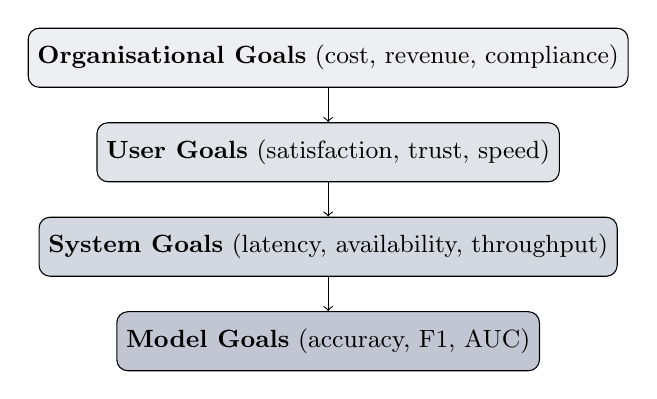
\begin{tikzpicture}[font=\small,every node/.style={draw,rounded corners,minimum width=4cm,minimum height=0.75cm,align=center}]
  \node[fill=navy!8] (org) at (0,4) {\textbf{Organisational Goals} (cost, revenue, compliance)};
  \node[fill=navy!14] (user) at (0,2.8) {\textbf{User Goals} (satisfaction, trust, speed)};
  \node[fill=navy!20] (sys) at (0,1.6) {\textbf{System Goals} (latency, availability, throughput)};
  \node[fill=navy!28] (model) at (0,0.4) {\textbf{Model Goals} (accuracy, F1, AUC)};
  \draw[->] (org)--(user); \draw[->] (user)--(sys); \draw[->] (sys)--(model);
\end{tikzpicture}
\end{center}

\begin{intuition}
Think of it as a telescope: each lens must be aligned for the final image to be clear. If the model is accurate but the system is slow, users are unhappy. If users are happy but the system is expensive, the business is unhappy. All four lenses must point in the same direction.
\end{intuition}

\begin{worked}{Goal alignment in the credit risk system}
A bank wants to approve loan applications faster while reducing default rates. The goal alignment looks like: \\[4pt]
\textbf{Organisational goal:} Reduce loan default rate by 15\,\% over 12 months; reduce manual review cost by 40\,\%. \\
\textbf{User goal (loan officer):} Get a risk score with explanation within 10 seconds of submitting application. \\
\textbf{System goal:} Process risk scoring API in under 2 seconds at 99.9\,\% availability. \\
\textbf{Model goal:} Achieve AUC $\geq$ 0.85 on held-out test set; false negative rate $\leq$ 5\,\% (do not miss true defaults). \\[4pt]
Notice: the model goal is \emph{derived} from the organisational and user goals. You cannot define the model goal without knowing the business and user goals.
\end{worked}

\begin{watchout}
Optimising only the model goal (AUC) while ignoring system goals (latency) is a classic RE mistake. A model with AUC 0.92 that takes 30 seconds to respond is useless if the loan officer is waiting at the counter with a customer.
\end{watchout}

%==============================================================
\section{GR4ML: Business View}
%==============================================================

\vocab{GR4ML} (Goal and Requirement for ML) is a formal modelling notation that connects high-level business goals to specific ML components. It has three views: Business, Analytics Design, and Data Preparation.

The \vocab{Business View} models the organisational context of the ML system.

\begin{center}
\resizebox{\linewidth}{!}{%
\begin{tabular}{lll}
\toprule
\textbf{Element} & \textbf{Meaning} & \textbf{Credit risk example} \\
\midrule
Actor & Stakeholder who drives decisions & Case Worker (loan officer) \\
StrategicGoal & High-level business objective & Make good lending decisions \\
DecisionGoal & Specific decision to fulfill the strategy & Approve or reject this loan application \\
QuestionGoal & Question that must be answered to decide & What is the credit risk of this applicant? \\
Insight & Data-driven answer to the question & Credit risk score: 0.73 (high risk) \\
Indicator & Metric measuring if the goal is achieved & Loan default rate (\%) \\
UpdateFrequency & How often the model runs & Monthly (batch retraining) \\
LearningPeriod & Historical window used for training & Last 24 months of loan data \\
\bottomrule
\end{tabular}}
\end{center}

\begin{intuition}
The Business View is a ``why'' map. It traces the chain from ``why do we need this ML system at all'' (StrategicGoal) down to ``what specific number does the ML model produce'' (Insight). This chain ensures every ML decision can be justified by a business need.
\end{intuition}

%==============================================================
\section{GR4ML: Analytics Design View}
%==============================================================

The \vocab{Analytics Design View} specifies what kind of analytical task the ML component performs and which quality attributes guide the algorithm choice.

\begin{center}
\resizebox{\linewidth}{!}{%
\begin{tabular}{lll}
\toprule
\textbf{Element} & \textbf{Meaning} & \textbf{Example} \\
\midrule
AnalyticsGoal & The type of insight to generate & PredictionGoal: predict default probability \\
PredictionGoal & Forecast future/unknown outcome & Will this applicant default? \\
DescriptionGoal & Understand or summarise data & Which customer segments default most? \\
PrescriptionGoal & Recommend optimal action & Which loan terms minimise expected loss? \\
Algorithm & Computational method chosen & Gradient Boosted Trees (XGBoost) \\
SoftGoal (Interpretability) & Loan officers must explain decisions to customers & High weight given to explainability \\
SoftGoal (Accuracy) & Regulatory requirement: AUC $\geq$ 0.85 & High weight given to predictive power \\
\bottomrule
\end{tabular}}
\end{center}

\begin{worked}{Analytics design trade-off}
The bank's credit risk model must be both \emph{accurate} (minimise defaults) and \emph{interpretable} (loan officers must explain rejections to customers --- a regulatory requirement). \\[4pt]
XGBoost achieves AUC 0.88 but is a black box. A logistic regression achieves AUC 0.81 but is fully interpretable. \\[4pt]
\textbf{Decision:} Use XGBoost with SHAP (SHapley Additive exPlanations) values. SHAP produces an explanation: ``This application was rejected primarily because debt-to-income ratio (45\,\%) exceeds the threshold (35\,\%), and credit utilisation (82\,\%) is very high.'' This satisfies both SoftGoals.
\end{worked}

%==============================================================
\section{GR4ML: Data Preparation View}
%==============================================================

The \vocab{Data Preparation View} maps the raw data sources to the clean, feature-engineered dataset that the model will train on.

Key elements:
\begin{itemize}
  \item \vocab{Entity} --- data objects (tables, APIs, files): \texttt{LoanApplication}, \texttt{CreditBureau}, \texttt{TransactionHistory}.
  \item \vocab{DataPreparationTask} --- operations: Data Cleaning, Data Reduction, Normalisation, Encoding.
  \item \vocab{Operator} --- specific method: remove rows with missing income (cleaning), min-max scale loan amount (normalisation), one-hot encode loan purpose (encoding).
  \item \vocab{Mechanism} --- implementation: Python/pandas, Apache Spark, SQL.
\end{itemize}

\begin{worked}{Data preparation for credit risk}
\textbf{Input:} Raw tables --- LoanApplication (50 columns), CreditBureau (30 columns), 3 years of TransactionHistory. \\[4pt]
\textbf{Task 1 (Cleaning):} Remove 3{,}200 rows with missing annual income (3.2\,\% of records). Impute 800 rows with missing credit score using median by age bracket. \\
\textbf{Task 2 (Reduction):} Drop 22 columns with $>$40\,\% missing values. Retain 35 predictive features. \\
\textbf{Task 3 (Normalisation):} Min-max scale: loan\_amount, annual\_income, total\_debt (to bring all to $[0,1]$). \\
\textbf{Task 4 (Encoding):} One-hot encode: loan\_purpose (12 categories $\rightarrow$ 12 binary columns), employment\_type (4 categories). \\
\textbf{Output:} 97{,}000 clean rows, 58 features, ready for XGBoost training.
\end{worked}

%==============================================================
\section{Measuring Goals: Measures and Metrics}
%==============================================================

A \vocab{measure} is the method or standard used to quantify something. A \vocab{metric} is the actual measured value. A good measure: directly relates to a goal, is quantifiable and objective, and is practical to collect.

\begin{everyday}
A measure for ``good health'' might be blood pressure, body temperature, and resting heart rate. The metric for your blood pressure today is 120/80 mmHg. The goal (good health) is abstract; the measure (blood pressure) makes it concrete; the metric (120/80) tells you where you stand today.
\end{everyday}

\begin{worked}{Chatbot goal to measures}
\textbf{Goal:} ``Improve chatbot usefulness.'' \\[4pt]
\textbf{Measure 1:} Task success rate --- fraction of conversations in which the user's intent was fulfilled. \\
\textbf{Measure 2:} User satisfaction score (1--5 stars, collected post-chat). \\
\textbf{Measure 3:} Conversation completion rate --- fraction of users who did not abandon mid-conversation. \\
\textbf{Measure 4:} Escalation rate --- fraction of conversations escalated to a human agent (lower is better). \\[4pt]
Notice that ``improve chatbot usefulness'' is unmeasurable by itself. Only after you define the four measures can you set targets, run experiments, and know if you are improving.
\end{worked}

%==============================================================
\section{Accuracy vs Precision of Measurement}
%==============================================================

These two words are often confused. They describe independent properties of a measurement system.

\begin{itemize}
  \item \vocab{Accuracy} --- how close the measured value is to the true value.
  \item \vocab{Precision} --- how consistently the measurement produces the same result when repeated.
\end{itemize}

\begin{intuition}
Think of darts. Accurate = clustered around the bullseye. Precise = clustered tightly together (but may be far from the bullseye). The ideal is both: tight cluster, centred on the bullseye. The worst is neither: scattered all over.
\end{intuition}

\begin{worked}{Thermometer accuracy and precision}
True body temperature: $98.6^\circ$F. We take five measurements with two thermometers: \\[4pt]
\textbf{Thermometer A} (precise, not accurate): $[98.2, 98.1, 98.3, 98.2, 98.1]$ \\
Mean = $98.18^\circ$F. Bias = $-0.42^\circ$F. Std dev = $0.08^\circ$F. \\
Verdict: very consistent (low std dev) but systematically off (high bias). Calibration can fix this. \\[4pt]
\textbf{Thermometer B} (accurate, not precise): $[98.4, 99.1, 97.9, 98.8, 99.2]$ \\
Mean = $98.68^\circ$F. Bias = $+0.08^\circ$F. Std dev = $0.53^\circ$F. \\
Verdict: centred on the right value (low bias) but noisy (high std dev). Hard to rely on for a single reading. \\[4pt]
\textbf{In ML:} A model with high precision/low variance makes consistent predictions; high accuracy/low bias means those predictions are correct. Both matter. Bias--variance trade-off is the ML counterpart of accuracy--precision.
\end{worked}

\begin{keytake}
Precision without accuracy is measuring the wrong thing reliably. Accuracy without precision means you cannot trust any single measurement. You need both.
\end{keytake}

\end{document}
